\documentclass[xcolor=svgnames]{beamer}\usepackage[]{graphicx}\usepackage[]{color}
%% maxwidth is the original width if it is less than linewidth
%% otherwise use linewidth (to make sure the graphics do not exceed the margin)
\makeatletter
\def\maxwidth{ %
  \ifdim\Gin@nat@width>\linewidth
    \linewidth
  \else
    \Gin@nat@width
  \fi
}
\makeatother

\definecolor{fgcolor}{rgb}{0.345, 0.345, 0.345}
\newcommand{\hlnum}[1]{\textcolor[rgb]{0.686,0.059,0.569}{#1}}%
\newcommand{\hlstr}[1]{\textcolor[rgb]{0.192,0.494,0.8}{#1}}%
\newcommand{\hlcom}[1]{\textcolor[rgb]{0.678,0.584,0.686}{\textit{#1}}}%
\newcommand{\hlopt}[1]{\textcolor[rgb]{0,0,0}{#1}}%
\newcommand{\hlstd}[1]{\textcolor[rgb]{0.345,0.345,0.345}{#1}}%
\newcommand{\hlkwa}[1]{\textcolor[rgb]{0.161,0.373,0.58}{\textbf{#1}}}%
\newcommand{\hlkwb}[1]{\textcolor[rgb]{0.69,0.353,0.396}{#1}}%
\newcommand{\hlkwc}[1]{\textcolor[rgb]{0.333,0.667,0.333}{#1}}%
\newcommand{\hlkwd}[1]{\textcolor[rgb]{0.737,0.353,0.396}{\textbf{#1}}}%

\usepackage{framed}
\makeatletter
\newenvironment{kframe}{%
 \def\at@end@of@kframe{}%
 \ifinner\ifhmode%
  \def\at@end@of@kframe{\end{minipage}}%
  \begin{minipage}{\columnwidth}%
 \fi\fi%
 \def\FrameCommand##1{\hskip\@totalleftmargin \hskip-\fboxsep
 \colorbox{shadecolor}{##1}\hskip-\fboxsep
     % There is no \\@totalrightmargin, so:
     \hskip-\linewidth \hskip-\@totalleftmargin \hskip\columnwidth}%
 \MakeFramed {\advance\hsize-\width
   \@totalleftmargin\z@ \linewidth\hsize
   \@setminipage}}%
 {\par\unskip\endMakeFramed%
 \at@end@of@kframe}
\makeatother

\definecolor{shadecolor}{rgb}{.97, .97, .97}
\definecolor{messagecolor}{rgb}{0, 0, 0}
\definecolor{warningcolor}{rgb}{1, 0, 1}
\definecolor{errorcolor}{rgb}{1, 0, 0}
\newenvironment{knitrout}{}{} % an empty environment to be redefined in TeX

\usepackage{alltt}
\usetheme{Boadilla}
\usecolortheme[named=SeaGreen]{structure}
\usepackage{graphicx}
\usepackage{breqn}
\usepackage{xcolor}
\usepackage{booktabs}
\usepackage{verbatim}
\usepackage{tikz}
\usepackage{lmodern}
\usetikzlibrary{shadows,arrows,positioning}
\definecolor{links}{HTML}{2A1B81}
\hypersetup{colorlinks,linkcolor=links,urlcolor=links}
\usepackage{pgfpages}

\newcommand{\Bigtxt}[1]{\textbf{\textit{#1}}}
\IfFileExists{upquote.sty}{\usepackage{upquote}}{}
\begin{document}

\title[Group Activity]{Group Activity}

\author[M. Beck, T. O'Brien]{Marcus W. Beck\inst{1} \and Todd D. O'Brien\inst{2}}

\date{}

\institute[]{\inst{1} ORISE, USEPA NHEERL Gulf Ecology Division\\ Email: \href{mailto:beck.marcus@epa.gov}{beck.marcus@epa.gov} \and \inst{2} NOAA/NMFS COPEPOD Project\\ Email: \href{todd.obrien@noaa.gov}{todd.obrien@noaa.gov}}

% knitr setup


% load SWMPr from local


%%%%%%
\begin{frame}
\vspace{0.3in}
\centerline{
\begin{tikzpicture}
  \node[drop shadow={shadow xshift=0ex,shadow yshift=0ex},fill=white,draw] at (0,0) {
\includegraphics[width=0.9\textwidth]{bg_main.jpg}};
\end{tikzpicture}}
\titlepage
\end{frame}

%%%%%%
\begin{frame}{Objectives and agenda}
\begin{itemize}
\item Objectives \\~\\
\begin{itemize}
\item Participants should be comfortable retrieving, organizing, and analyzing a SWMP dataset \\~\\
\item Understand the questions and use appropriate methods\\~\\
\end{itemize}
\item Agenda \\~\\
\begin{itemize}
\item Dataset description and questions \\~\\
\item Group activity
\end{itemize}
\end{itemize}
\end{frame}

%%%%%%
\begin{frame}{Dataset description}
Hurricane Sandy
\begin{columns}
\begin{column}{0.45\textwidth}
\begin{itemize}
\item Largest Altantic hurricane on record (by  diameter)
\item Second costliest US hurricane
\item US landfall October 29\textsuperscript{th}, 2012
\item Cat 2 on landfall
\item Rainfall exceeding 12 inches, 13 foot storm surge in some areas
\end{itemize}
\end{column}
\begin{column}{0.45\textwidth}
\centerline{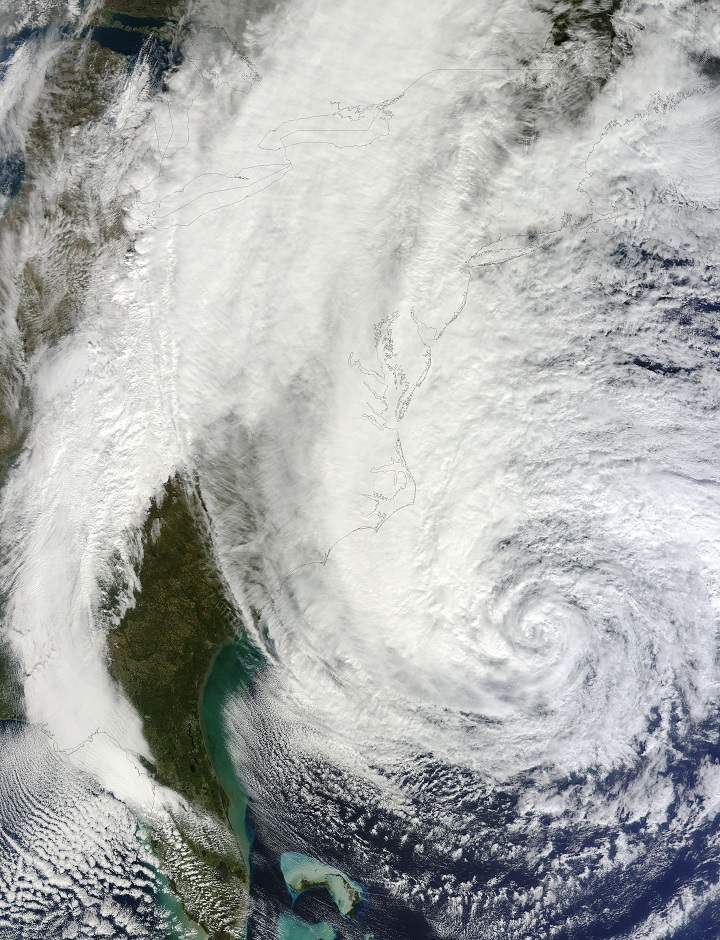
\includegraphics[width = 0.9\textwidth]{Sandy_Oct_28_2012.jpg}}
\end{column}
\end{columns}
\end{frame}

%%%%%%
\begin{frame}{Dataset description}
Several NERRS reserves were impacted, landfall directly over Jacques Cousteau
\centerline{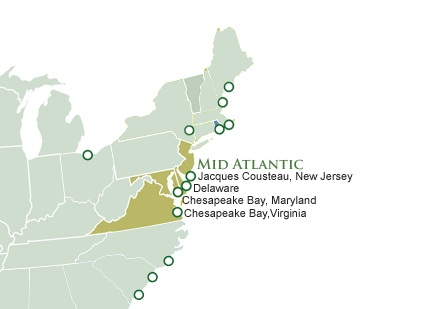
\includegraphics[width = 0.7\textwidth]{mid_atlantic.jpg}}
\end{frame}

%%%%%%
\begin{frame}{Dataset description}
We will look at the water quality, nutrients, and weather data for 2012 and 2013 for Jacques Cousteau -- `dataset4' folder \\~\\
\begin{block}{Overall question}
How did the hurricane impact the reserve?
\end{block}
\vspace{0.1in}
Specific questions
\begin{itemize}
\item Are there noticeable changes in the time series? Which parameters?
\item Are the long-term means different before and after landfall?
\item Can the effects be detected prior to landfall?
\item How long did the effects persist after the storm?
\end{itemize}
\end{frame}

%%%%%%
\begin{frame}{Dataset description}
Specific questions
\begin{itemize}
\item Are there noticeable changes in the time series? Which parameters?
\item Are the long-term means different before and after landfall?
\item Can the effects be detected prior to landfall?
\item How long did the effects persist after the storm? \\~\\
\end{itemize}
How will you address these questions?
\begin{itemize}
\item What parameters or stations will you consider?
\item How will you subset, combine, aggregate?
\item What plots will you create?
\item How will you interpret your results? \\~\\
\end{itemize}
Resources - cookbook, SWMPr tutorial, instructors, your table buddies!
\end{frame}

%%%%%%
\begin{frame}
\vspace{0.3in}
\centerline{
\begin{tikzpicture}
  \node[drop shadow={shadow xshift=0ex,shadow yshift=0ex},fill=white,draw] at (0,0) {
\includegraphics[width=0.9\textwidth]{bg_main.jpg}};
\end{tikzpicture}}
\vspace{0.5in}
\Large
\centerline{\Bigtxt{Questions??}}
\end{frame}

\end{document}
